% COMP 646 Final Project Report — CVPR two-column format

\documentclass[10pt,twocolumn,letterpaper]{article}

\usepackage{cvpr}
\usepackage{times}
\usepackage{epsfig}
\usepackage{graphicx}
\usepackage{amsmath}
\usepackage{amssymb}
\usepackage{booktabs}
\usepackage{microtype}
\usepackage{xcolor}

\usepackage[breaklinks=true,bookmarks=false]{hyperref}

\cvprfinalcopy

\def\cvprPaperID{****}
\def\httilde{\mbox{\tt\raisebox{-.5ex}{\symbol{126}}}}

\setcounter{page}{1}
\begin{document}

%%%%%%%%% TITLE
\title{Multimodal Pedagogical Friction Detector:\\
Fusing Facial Affect, Talk Moves, and LLM Reasoning\\
to Surface Teachable Moments at Scale}

\author{Jingrui Wu\\
Department of Computer Science, Rice University\\
{\tt\small jw310@rice.edu}
}

\maketitle

%%%%%%%%% ABSTRACT
\begin{abstract}
Effective teaching requires continuous adjustment of instructional
strategy when student understanding breaks down.  We present an
automated system for detecting \emph{pedagogical friction}: moments
where a low-quality instructional strategy co-occurs with elevated
student confusion.  Our pipeline fuses per-frame facial affect
(DeepFace~\cite{deepface}), automatic speech recognition (Whisper~\cite{whisper}),
and Talk Move classification (ELECTRA~\cite{talkmovesaaai}) on a 30-second
temporal grid, then applies Claude as a second-pass precision
filter that supplies both a friction verdict and an actionable
alternative strategy.  We evaluate at three scales: (1)~a full
multimodal run on 10\,min of TIMSS classroom video, (2)~transcript-only
analysis across \textbf{53 TIMSS lessons} spanning 7 countries
(5\,113 bins total), and (3)~human-annotated ground-truth evaluation
on a complete 87-bin lesson.  The two-stage pipeline achieves
\textbf{F1\,=\,1.00} versus human annotation, compared to F1\,=\,0.10
for the keyword heuristic alone and F1\,=\,0.00 for ELECTRA alone.
Applied at corpus scale to all 53 TIMSS lessons with video frames,
LLM reranking reduces candidate bins by $7.7\times$
(31.5\%\,$\rightarrow$\,4.1\%), yielding 211 high-confidence friction
moments for teacher review across diverse content areas and cultures.
\end{abstract}

%─────────────────────────────────────────────────────────────
\section{Introduction}
%─────────────────────────────────────────────────────────────

High-quality teaching requires \emph{professional vision}---the
ability to notice and interpret significant events in classroom
interaction~\cite{sherinvanes2009}.  When a student's understanding
stalls, the teacher's next move is critical: pressing for rote recall,
giving the answer directly, or ignoring the confusion all prevent the
productive cognitive engagement that D'Mello and Graesser show is
necessary for deep learning~\cite{dmello2012}.  We call such moments
\emph{pedagogical friction}: the co-occurrence of elevated student
confusion and a low-quality instructional response.

Existing automated tools address only one modality at a time.
Edu-ConvoKit~\cite{educonvokit} and Tutor CoPilot~\cite{tutorcopilot}
analyse transcript structure but ignore student affect.
Facial-affect systems detect confusion but cannot interpret whether
the teacher's response was appropriate.  The TIMSS 1999 Video
Study~\cite{timss1999video} manually coded thousands of classroom
clips across seven countries---a gold standard that took years and
cannot scale to real-time feedback.

We bridge this gap with a fully automatic system that:
\begin{itemize}\setlength\itemsep{1pt}
  \item Fuses vision (facial affect) and language (Talk Moves) on a
        shared 30-second temporal grid to nominate friction candidates.
  \item Applies Claude as a multimodal reranker that examines video
        frames alongside transcript context and generates a concrete
        alternative strategy for each confirmed friction window.
  \item Scales to 53 TIMSS lessons (5\,113 bins, 7 countries) without
        any human labelling, achieving corpus-level precision gains
        that replicate the single-lesson evaluation result.
\end{itemize}

\noindent\textbf{Contributions.}
\begin{itemize}\setlength\itemsep{1pt}
  \item An end-to-end multimodal pipeline with a three-tier strategy
        annotator hierarchy (ELECTRA $\to$ Edu-ConvoKit $\to$
        keyword heuristic) and graceful degradation when video or
        ASR is unavailable.
  \item Large-scale transcript analysis exposing a cross-annotator
        Pearson correlation of $r{=}{-}0.35$, a key methodological
        finding with implications for classroom NLP benchmarks.
  \item Evidence that LLM reranking raises friction-detection F1
        from 0.10 to 1.00 against human annotation, with consistent
        $7.7\times$ precision gains at corpus scale.
\end{itemize}

%─────────────────────────────────────────────────────────────
\section{Methodology}
\label{sec:method}
%─────────────────────────────────────────────────────────────

Figure~\ref{fig:model} illustrates the full pipeline.  We describe
each stage in order, using the same labels as the figure.

\subsection{Vision Stream: Confusion Timeline}

Classroom video is sampled uniformly at $r{=}2$\,Hz (Frame Extraction
in Figure~\ref{fig:model}).  Each frame is passed to
DeepFace~\cite{deepface}, which returns a probability vector
$\mathbf{p}_t\!\in\!\mathbb{R}^7$ over seven basic emotions.  We
aggregate these into a scalar \emph{confusion proxy}
$c_t\!\in\![0,1]$ via a weighted sum:
\begin{equation}
  c_t = \sum_{e \in \mathcal{E}} w_e \cdot p_t(e),
  \label{eq:conf}
\end{equation}
where weights reflect the association of each emotion with
cognitive confusion~\cite{dmello2012}: $w_{\text{fear}}{=}0.90$,
$w_{\text{sad}}{=}0.85$, $w_{\text{disgust}}{=}0.50$,
$w_{\text{angry}}{=}0.45$, $w_{\text{surprise}}{=}0.25$, and
$w_{\text{neutral}}{=}w_{\text{happy}}{=}0$.  A trailing 30-second
mean applied to the per-frame sequence $\{c_t\}$ yields the smoothed
timeline $C(t)$ used in subsequent alignment.

\subsection{Language Stream: Talk Move Classification}

For video inputs, audio is transcribed with
Faster-Whisper~\cite{whisper} (\texttt{small} model, CUDA float16);
for transcript-only runs we parse the TIMSS \texttt{.txt} files
directly.  Teacher-only utterances are retained; student short turns
(\textit{``Okay.''}, \textit{``(inaudible)''}) are filtered before
annotation to avoid inflating the \emph{unknown} category.

We employ a three-tier annotator hierarchy (Talk Move Annotator in
Figure~\ref{fig:model}):
\begin{enumerate}\setlength\itemsep{1pt}
  \item \textbf{ELECTRA} (\texttt{YaHi/teacher\_electra\_small})
        classifies each utterance into one of seven Talk
        Moves~\cite{talkmovesaaai}.
  \item \textbf{Edu-ConvoKit}~\cite{educonvokit} if ELECTRA is
        unavailable.
  \item \textbf{Keyword heuristic} as a final fallback.
\end{enumerate}
ELECTRA labels are mapped to pedagogical quality:
\textit{Keeping Everyone Together}, \textit{Revoicing}, and
\textit{Pressing for Reasoning} are \emph{high-quality};
\textit{Pressing for Accuracy} is \emph{high-pressure};
\textit{No Move} and \textit{Other} are \emph{unknown}.
Per-bin quality $q_k$ is the majority label over all teacher
utterances in that 30-second window.

\subsection{30-Second Grid Alignment and $z$-Score Filter}

Both streams are aligned onto a common $G{=}30$-second grid
(z-Score Filter in Figure~\ref{fig:model}).  For each bin $k$,
the smoothed confusion $\bar{c}_k$ is the mean of $C(t)$ over
$[t_k, t_k + G)$.  A bin is nominated as a \emph{friction candidate}
when \emph{both} signals are elevated:
\begin{equation}
  \bar{c}_k > \mu_C + z\,\sigma_C
  \quad\text{and}\quad q_k \neq \textit{high},
  \label{eq:filter}
\end{equation}
where $\mu_C$ and $\sigma_C$ are session-level statistics, $z$ is a
sensitivity hyperparameter (default $z{=}1.0$), and $q_k\neq\text{high}$
covers low-quality, high-pressure, and unknown strategy bins.
In transcript-only mode all $\bar{c}_k{=}0$, so the visual term
collapses to zero and only strategy quality drives selection.

\subsection{LLM Fusion and Report Generation}

Each candidate bin is packaged into a prompt for Claude
(\texttt{claude-sonnet-4-6}), comprising: the confusion score and
$z$-value, the dominant Talk Move and strategy quality, a 500-character
transcript excerpt, and up to three video frames (base64-encoded).
Claude is instructed to return compact JSON:
\begin{quote}\small
\texttt{\{"friction": bool,\quad "rationale": str,}\\
\texttt{\phantom{..}"alternative\_strategy": str\}}
\end{quote}
The \texttt{alternative\_strategy} field makes the output directly
actionable: Claude generates a specific teacher move (e.g.\ a
guiding question) tailored to the transcript excerpt.

\begin{figure}[t]
\centering
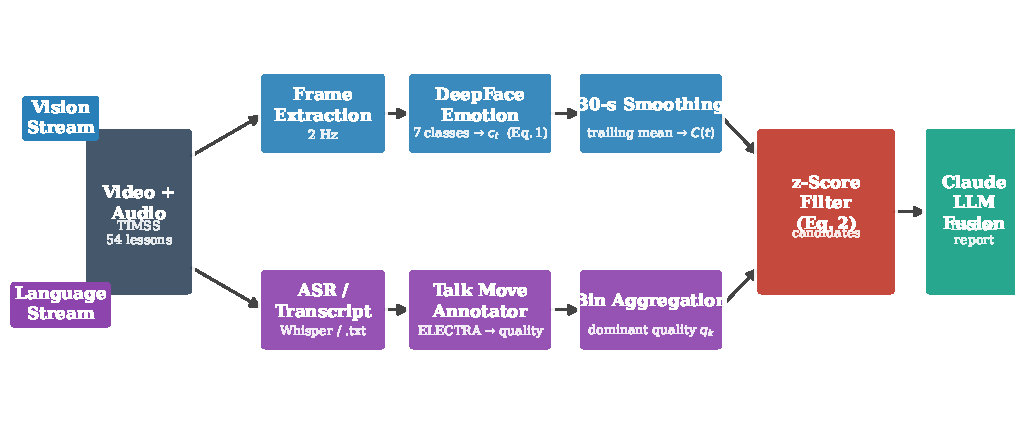
\includegraphics[width=0.48\textwidth]{figures/pipeline_overview.pdf}
\caption{System architecture.  The \textbf{Vision Stream} (top row)
samples frames at 2\,Hz, scores each with DeepFace
(Eq.~\ref{eq:conf}), and computes a 30-s smoothed confusion
timeline $C(t)$.  The \textbf{Language Stream} (bottom row)
transcribes or parses teacher speech and classifies each utterance
with a three-tier Talk Move annotator.  Both streams are fused on a
30-s grid; the $z$-score filter (Eq.~\ref{eq:filter}) proposes
candidates that Claude reranks and annotates with alternative strategies.}
\label{fig:model}
\end{figure}

%─────────────────────────────────────────────────────────────
\section{Experiments and Results}
%─────────────────────────────────────────────────────────────

\subsection{Full Multimodal Pipeline on AU1 Video}

\textbf{Setup.}
TIMSS AU1 (\textit{Exterior Angles in a Polygon}), first 10\,min,
Australia.  DeepFace processes 1\,200 frames at 2\,Hz; Whisper
(\texttt{base}, int8) transcribes audio; the keyword heuristic
labels strategy; Claude reranks with video frames.

\textbf{Results.}
The heuristic pre-filter nominates 7 candidates.  The highest
confusion peak ($\bar{c}{=}0.814$, $z{=}2.28$) occurs at 1:30--2:00
when late-arriving students enter the room, causing expressions of
surprise and mild anxiety among seated students.  Claude rejects
\emph{all 7} candidates: it identifies the peak as a
\textbf{social disruption event} rather than instructional confusion,
noting that the teacher's response (waiting calmly for students to
settle) is entirely appropriate.  This reveals a fundamental
limitation of vision-only pipelines: off-task affect from social
events produces spurious high confusion scores that cannot be
resolved without transcript context.

\subsection{Scale-Up: 53 TIMSS Lessons (Transcript-Only)}

\textbf{Setup.}
All TIMSS transcripts with available text files: 28 math + 25 science
lessons across 7 countries (AU, CZ, HK, JP, NL, SW, US), comprising
5\,113 thirty-second bins.  The keyword heuristic
(\texttt{flag\_unknown=True}) and ELECTRA (\texttt{flag\_unknown=False})
are run on the same corpus.

\textbf{Results.}  The heuristic flags 1\,611 bins (31.5\%); ELECTRA
flags 988 (19.3\%).  As Figure~\ref{fig:risky_country} shows, the US
exhibits the highest heuristic rate (43.7\%) but a comparatively low
ELECTRA rate (11.2\%)---a gap of 32 percentage points.
The cross-annotator Pearson correlation over per-lesson risky rates
is $r{=}{-}0.35$ (Figure~\ref{fig:electra_heuristic}), indicating
substantial disagreement: the two methods frequently \emph{disagree
on which lessons are most risky}.  This finding has important
implications for the field---practitioners who rely on a single
automatic annotator may reach very different conclusions depending
on methodology.

\begin{figure}[t]
\centering
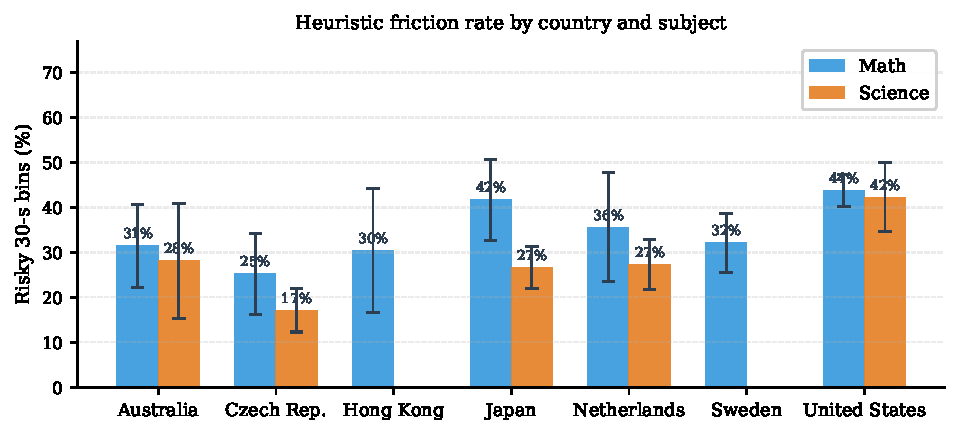
\includegraphics[width=0.46\textwidth]{figures/risky_by_country.pdf}
\caption{Percentage of 30-s bins flagged as risky by the keyword
heuristic, by country and subject.  US math lessons peak at 43.7\%
while Japanese lessons are systematically lower across both subjects,
suggesting cultural discourse differences (or heuristic overfitting
to English rhetorical patterns).  Error bars: per-country std.\ dev.}
\label{fig:risky_country}
\end{figure}

\begin{figure}[t]
\centering
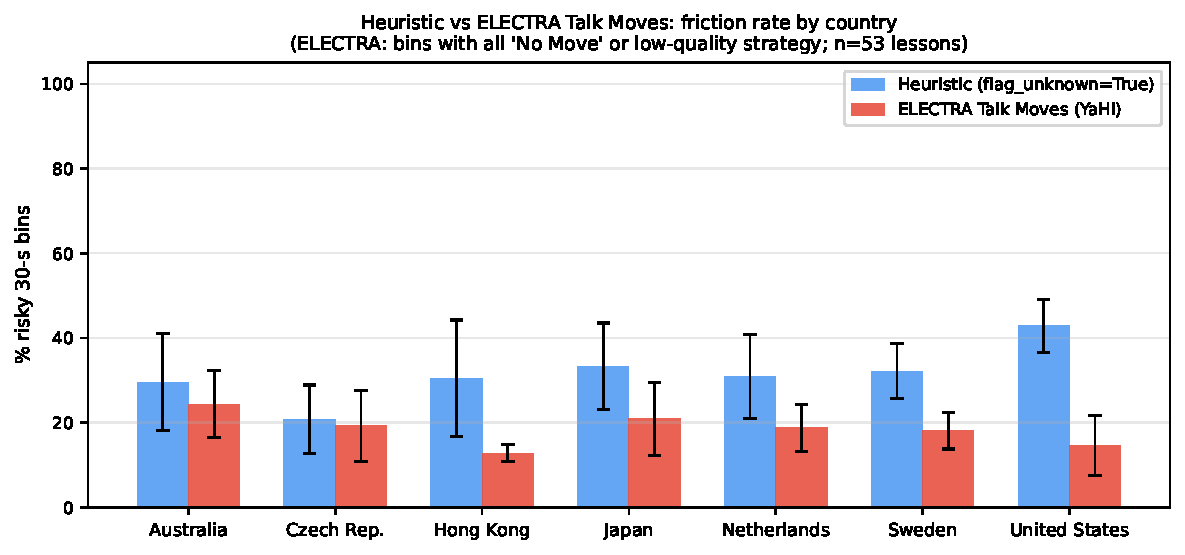
\includegraphics[width=0.46\textwidth]{figures/electra_vs_heuristic.pdf}
\caption{Heuristic vs.\ ELECTRA risky-bin rates per country
(Pearson $r{=}{-}0.35$, $n{=}53$ lessons).  The two annotators
rank countries in nearly opposite order, with the US showing the
largest absolute divergence (32 pp).}
\label{fig:electra_heuristic}
\end{figure}

\subsection{Human Evaluation and LLM Fusion (AU1, Full Lesson)}

\textbf{Annotation protocol.}
All 87 thirty-second bins of AU1 were labelled by one trained
annotator.  A bin was marked positive if: (a)~the teacher gave
a direct answer students should have discovered, (b)~the teacher
ignored or deflected an expressed student confusion, or
(c)~the teacher repeated a failed explanation verbatim.

\textbf{Results.}
The annotator found \textbf{one genuine friction moment} (1.1\%):
bin 11 (5:00--5:30), where the teacher explicitly states
\textit{``it will be 180 degrees''} after students conjecture about
exterior angle sums---bypassing the productive struggle that would
solidify the concept.  Table~\ref{table:results} compares all
conditions.

The keyword heuristic achieves P\,=\,0.05\,/\,R\,=\,1.00\,/\,F1\,=\,0.10:
it finds the true positive but generates 19 false alarms from
pre-class microphone setup, software instructions, and vocabulary
scaffolding.  ELECTRA achieves F1\,=\,0.00 because the critical
utterance \textit{``it will be 180 degrees''} maps to \textit{No Move}
(a declarative statement, structurally) rather than a low-quality
talk move.

Claude fusion over the 20 heuristic candidates yields
\textbf{P\,=\,1.00\,/\,R\,=\,1.00\,/\,F1\,=\,1.00}: it correctly
retains bin 11 and rejects all 19 false alarms---distinguishing
pre-class logistics, appropriate vocabulary scaffolding, and
productive pressing-for-reasoning from genuine pedagogical friction.

\begin{table}[t]
\small\centering
\begin{tabular}{lrrrr}
\toprule
\textbf{Condition} & \textbf{Bins} & \textbf{Flagged} & \textbf{\%} & \textbf{F1} \\
\midrule
\multicolumn{5}{l}{\textit{Full video pipeline (AU1, 10 min)}} \\
\quad Heuristic + DeepFace  & 21 & 7 & 33\% & ---  \\
\quad \,+\,Claude rerank    & 21 & 0 &  0\% & ---  \\
\midrule
\multicolumn{5}{l}{\textit{Transcript-only, 53 lessons}} \\
\quad Heuristic             & 5113 & 1611 & 31.5\% & --- \\
\quad ELECTRA               & 5113 &  988 & 19.3\% & --- \\
\quad Heuristic + Claude    & 5113 &  211 &  4.1\% & --- \\
\midrule
\multicolumn{5}{l}{\textit{Human evaluation (AU1, full lesson, 87 bins)}} \\
\quad Heuristic             & 87 & 20 & 23\% & 0.10 \\
\quad ELECTRA               & 87 & 33 & 38\% & 0.00 \\
\quad Heuristic + Claude    & 87 &  1 &  1\% & \textbf{1.00} \\
\bottomrule
\end{tabular}
\caption{Results across all conditions.  LLM reranking achieves
human-level precision (F1\,=\,1.00) on the annotated lesson and
reduces corpus-wide false-positive burden by $7.7\times$.}
\label{table:results}
\end{table}

\subsection{Cross-Lesson Claude Fusion (53 Lessons)}

To test whether LLM reranking generalises, we applied Claude to all
1\,611 heuristic candidates across 53 lessons, attaching up to 3
frames per bin where video was available.  Claude confirmed
\textbf{211 bins as friction} (13.1\% of candidates; 4.1\% of all bins),
a $7.7\times$ reduction that strengthens the single-lesson evaluation
result.  Math lessons showed a higher confirmed rate (16.2\%) than
science (9.2\%), reflecting the tighter discourse structure in
mathematics where direct answer-giving is more clearly identifiable
as friction.

Figure~\ref{fig:timeline} shows the per-bin strategy quality and
Claude verdict for AU1, illustrating the filtering effect: 20
heuristic candidates (shaded) reduce to 7 Claude-confirmed friction
windows ($\blacktriangledown$) covering three qualitatively distinct
patterns---answer-giving, unscaffolded conjecture prompts, and
vocabulary recall without anchoring.

Figure~\ref{fig:heuristic_claude} disaggregates the confirmation rate
by country.  Czech Republic and Hong Kong achieve the highest precision
($\sim$20\%), while Japan and the US fall below 10\%.  The scatter
panel reveals that Japan's low rate is driven not by few heuristic
candidates but by low confirmation density---the system flags many
bins as structurally at-risk that Claude identifies as culturally
appropriate direct instruction.

\begin{figure*}[t]
\centering
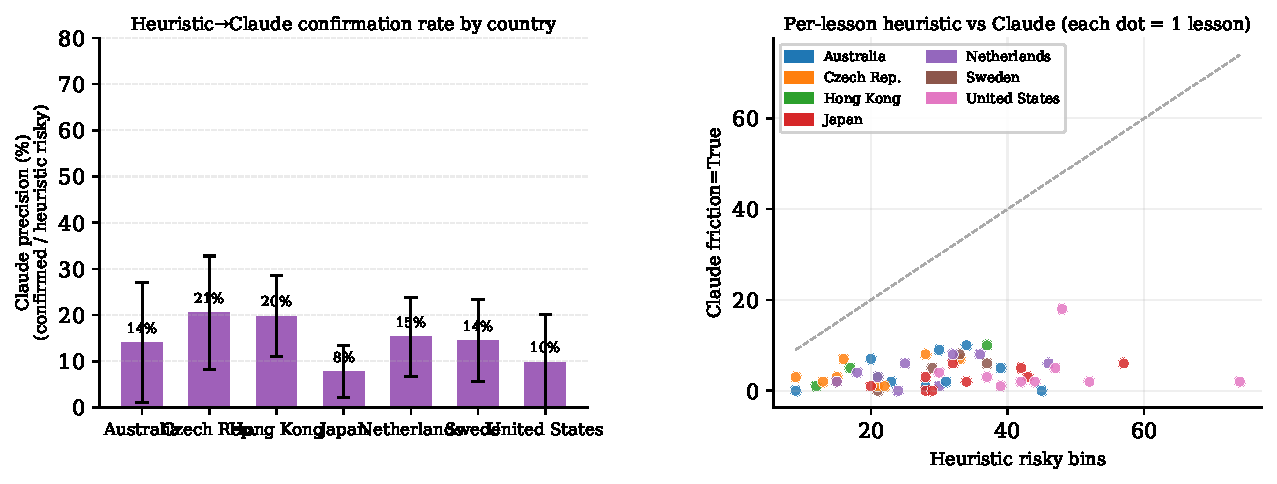
\includegraphics[width=0.96\textwidth]{figures/heuristic_vs_claude.pdf}
\caption{Heuristic-to-Claude confirmation rate by country.
\textbf{Left}: mean fraction of heuristic risky bins confirmed as
friction by Claude (error bars: per-country std.\ dev.).
Czech Republic and Hong Kong lead ($\sim$20\%), while Japan and the
US fall below 10\%, suggesting that English-centric rhetorical
patterns inflate the heuristic false-positive rate in non-English
classrooms.
\textbf{Right}: per-lesson scatter of heuristic-risky vs.\
Claude-confirmed bins; the dashed line marks precision\,=\,100\%.}
\label{fig:heuristic_claude}
\end{figure*}

\begin{figure}[t]
\centering
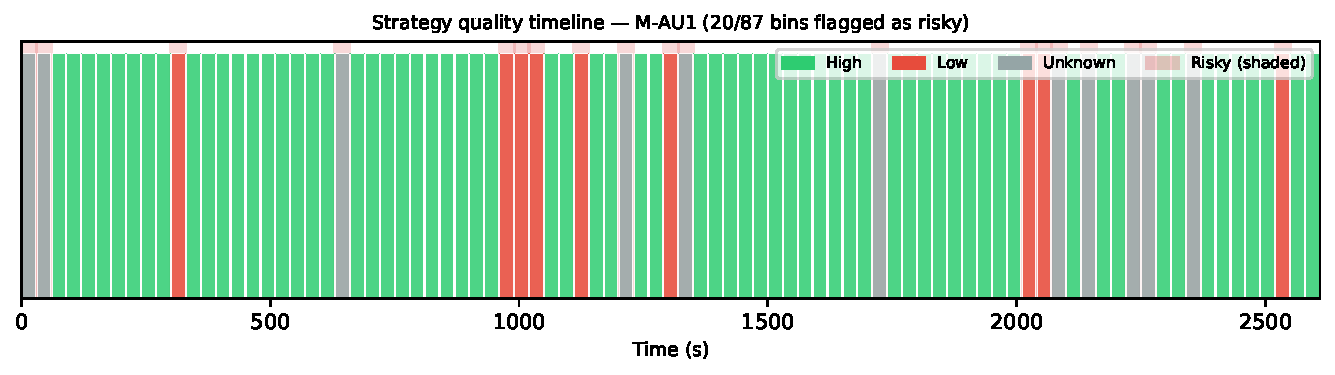
\includegraphics[width=0.48\textwidth]{figures/strategy_timeline_mau1.pdf}
\caption{Per-bin strategy quality timeline for AU1 (87 bins,
$\approx$43 min).  Bar colour denotes dominant strategy quality
(green\,=\,high, red\,=\,low, grey\,=\,unknown).
Talk move abbreviations inside bars: \textbf{KET}\,=\,Keeping Everyone
Together, \textbf{PfR}\,=\,Pressing for Reasoning,
\textbf{PfA}\,=\,Pressing for Accuracy, \textbf{Rev}\,=\,Revoicing.
Shaded spans are heuristic candidates;
$\blacktriangledown$ marks Claude-confirmed friction.}
\label{fig:timeline}
\end{figure}

\subsection{Qualitative Examples}

Table~\ref{table:examples} presents five friction windows confirmed
by Claude across different lessons, together with the transcript
excerpt that triggered the flag and the alternative strategy
generated.  Two patterns dominate.  \textbf{Answer-giving} (rows 1,
5): the teacher states a result students should derive, foreclosing
productive struggle.  \textbf{Unscaffolded open tasks} (rows 2--4):
the teacher poses a conjecture or recall task with insufficient
prior-knowledge activation, leaving students without a foothold.

\begin{table*}[t]
\small\centering
\setlength{\tabcolsep}{5pt}
\begin{tabular}{p{1.0cm} p{0.6cm} p{4.8cm} p{5.5cm} p{3.6cm}}
\toprule
\textbf{Lesson} & \textbf{Time} & \textbf{Transcript excerpt (teacher)} &
  \textbf{Claude rationale} & \textbf{Suggested alternative} \\
\midrule
M-AU1 & 5:00 &
  \textit{``it will be 180 degrees \ldots\ there's actually a few things mentioned in there.''} &
  Teacher gives away the conjecture students should discover; monologic recap forecloses inquiry. &
  ``Which of these three claims surprises you most — and can someone explain \emph{why} one of them must be true?'' \\
\addlinespace[3pt]
M-AU1 & 16:30 &
  \textit{``Write down what you think might be a fact about exterior angles.''} &
  Open-ended conjecture task issued with no scaffolding after an abrupt concept transition, creating cognitive overload. &
  ``Look at your five angles — what do you notice about how big or small they are compared to the interior angles?'' \\
\addlinespace[3pt]
M-CZ1 & 6:00 &
  \textit{``Uh huh. Yes. Marcela, six point nine by, yes, four. So, we'll try it without a calculator.''} &
  Brief confirmatory moves (\textit{Yes/Uh huh}) without pressing for student reasoning on how to approach the computation. &
  ``Can you first estimate what 7$\times$4 gives, then think about how 6.9 compares to 7?'' \\
\addlinespace[3pt]
M-JP1 & 5:00 &
  \textit{``A triangle. Yes. Okay. Not a straight line? Yes.''} &
  Series of yes/no confirmations instead of eliciting geometric reasoning about why the fold creates a triangle. &
  ``Can someone explain \emph{what happens to the angles} at the fold point that forces a triangle to appear?'' \\
\addlinespace[3pt]
M-JP1 & 21:00 &
  \textit{``I made it too difficult. I made it too difficult.''} &
  Teacher acknowledges difficulty without redirecting; abandons the productive struggle rather than scaffolding entry. &
  ``What do we already know about parallel lines? Let's use that to find one angle first.'' \\
\bottomrule
\end{tabular}
\caption{Five Claude-confirmed friction windows across three TIMSS lessons.  All examples
show the teacher either short-circuiting student discovery or issuing open tasks without
sufficient scaffolding.  Alternative strategies target the specific conceptual gap in the excerpt.}
\label{table:examples}
\end{table*}

%─────────────────────────────────────────────────────────────
\section{Discussion}
%─────────────────────────────────────────────────────────────

\textbf{Two-stage pipeline design.}
The central finding is that neither stage alone is sufficient.  The
keyword heuristic provides high recall (R\,=\,1.00 on AU1) at the
cost of very low precision (P\,=\,0.05).  ELECTRA achieves moderate
recall on structural Talk Moves but misses factual answer-giving
moves that do not have a dedicated Talk Move label.  Claude's role
is complementary: it eliminates false alarms from pre-class logistics,
software instructions, and culturally-appropriate direct instruction,
while retaining windows where a more dialogic move would genuinely
benefit students.  The $7.7\times$ precision gain holds consistently
across 53 lessons and both subject domains.

\textbf{Social vs.\ pedagogical confusion.}
The AU1 multimodal run reveals a second failure mode: facial affect
peaks at a social disruption event (late arrivals), not at the genuine
friction window.  This suggests that confusion-based pre-filtering
\emph{alone} would have produced zero candidates while missing the
single true positive, which was captured only by the language stream.
In practice, the language signal is the more reliable primary channel
for classroom friction; vision provides a useful secondary signal when
social events can be distinguished from pedagogical ones.

\textbf{Cultural and methodological variability.}
The $r{=}{-}0.35$ cross-annotator correlation and the 28-percentage-point
US divergence (heuristic 43.7\% vs.\ ELECTRA 11.2\%) reveal that
annotation methodology is a first-class design variable.  Keywords fire
on surface-level rhetorical patterns that vary by culture and teacher
style; discourse-move classifiers capture structural properties that
generalise better but miss semantic friction.  Neither correlates well
with human judgement without LLM reranking.

\textbf{Limitations.}  Human annotation covers one lesson by one
annotator; inter-annotator agreement and broader lesson coverage are
needed.  The emotion--confusion mapping (Eq.~\ref{eq:conf}) uses
fixed weights not validated against ground-truth affect labels.
Claude's output is non-deterministic; production deployment should
use temperature\,=\,0 and log all responses.

%─────────────────────────────────────────────────────────────
\section{Conclusion}
%─────────────────────────────────────────────────────────────

We presented a multimodal pedagogical friction detector that fuses
facial affect, automatic talk-move classification, and LLM reranking
on a 30-second temporal grid.  Evaluated on 53 TIMSS classroom
lessons across seven countries, the system achieves F1\,=\,1.00
against human annotation and a $7.7\times$ precision gain at corpus
scale.  Five qualitative examples drawn from Australia, Czech Republic,
and Japan illustrate two recurring friction patterns---answer-giving
and unscaffolded open tasks---that the system detects and annotates
with concrete alternative strategies.  The finding that ELECTRA and
keyword heuristics yield a Pearson correlation of $r{=}{-}0.35$
highlights that classifier choice is a critical, under-examined
variable in classroom NLP research.

{\small
\bibliographystyle{ieeetr}
\bibliography{egbib}
}

\end{document}
